%%
%  ******************************************************************************
%  * #file    Szablon_raportu_EN_Latex.tex
%  * #author  Adrian Wójcik   adrian.wojcik(at)put.poznan.pl
%  *          
%  * #commit  Patryk Kościk   koscikpatryk(at)gmail.com
%  *          Modified the template for Projekt przejsciowy purposes          
%  *          
%  *
%  * #commit  Patryk Kościk   koscikpatryk(at)gmail.com
%  *          Zupełnie przewrócono na łeb formatke po taktycznym wyjasnieniu          
%  *          
%  * #version 1.1
%  * #date    09-Mar-2022
%  * #brief   PROJPRZEJ
%  *
%  ******************************************************************************
%%  
\documentclass[11pt, a4paper]{article}

\usepackage{SM_template}

% Wypełnijcie te dyrektywy zgodnie z waszym tematem
%
% \lab      -> NAZWA CZUJNIKA,          np.: 'DHT22'
% \comment  -> Króciutki opis co to,    np.: 'Cyfrowy czujnik temperatury'
% \author   -> Autor dokumentu          np.: Patryk Kościk
%
% Pamiętajcie o zmianie ścieżki w \addbibresourcue (!)

\lab{SCOO 100ZP}
\comment{Przemysłowy optyczny czujnik obecności}
\author{Patryk Kościk}
\addbibresource{bib/KY-017.bib}

%
% Początek dokumentu
%
\begin{document}

%
% Strona tytułowa
%
\mainpage{SCOO/front-page.jpg}
\newpage

\section*{Opis elementu}
Metoda działania optycznego odbiciowego czujnika obecności opiera się na zjawisku refleksji światła. Detekcja przedmiotu czy substancji przez czujnik optyczny następuje w chwili gdy, wyemitowana wiązka światła, odbije się od przedmiotu (lub cieczy), aktywując wbudowany w czujnik detektor.



%%%%%%%%%%%%%%%%%%%%%%%%%  TWO IMAGES SIDE BY SIDE  %%%%%%%%%%%%%%%%%%%%%%%%%%%%%
\vspace{0.25cm}
\begin{figure}[h]
\centering
%%%%%%%%%%%%%%%%%%%%%%%%%%%%%%%%%%%%%%%%%%%%%%%%%%%%%%%%%%%%%%%%%%%%%%%%%%%%%%%%%
\begin{subfigure}{.5\textwidth}
\centering
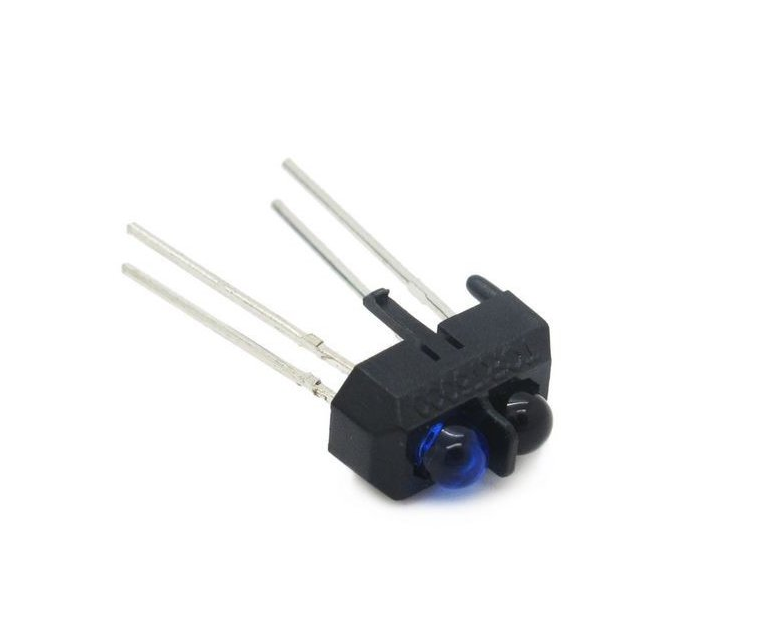
\includegraphics[width=.7\linewidth]{fig/SCOO/odb.png}
\caption{Zdjęcie zespołu optycznego sensora odbiciowego}
\label{fig:_zdjecie_elementu}
\end{subfigure}%
%%%%%%%%%%%%%%%%%%%%%%%%%%%%%%%%%%%%%%%%%%%%%%%%%%%%%%%%%%%%%%%%%%%%%%%%%%%%%%%%%
\begin{subfigure}{.5\textwidth}
\centering
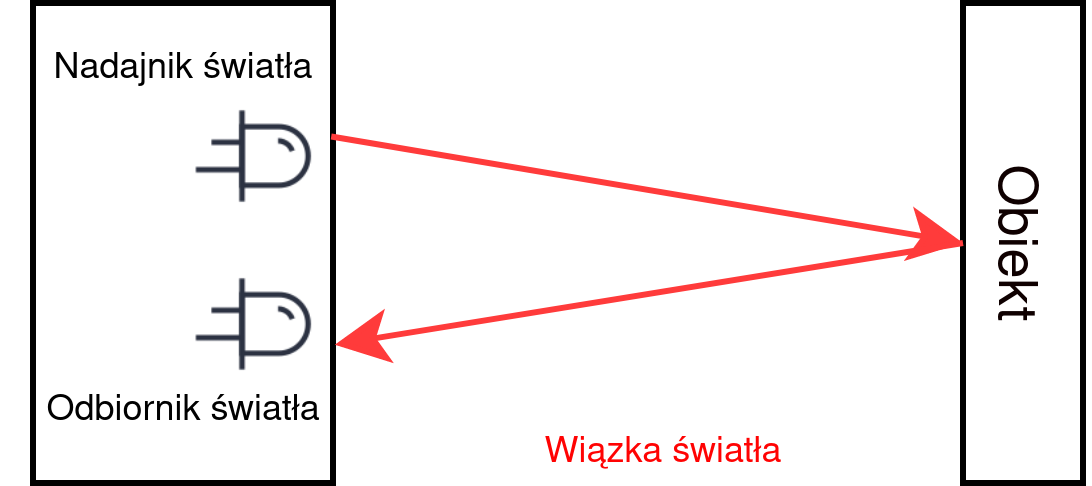
\includegraphics[width=.7\linewidth]{fig/SCOO/zasd.png}
\caption{Zasada działania sensora}
\label{fig:_zasada_dzialania_elementu}
\end{subfigure}
%%%%%%%%%%%%%%%%%%%%%%%%%%%%%%%%%%%%%%%%%%%%%%%%%%%%%%%%%%%%%%%%%%%%%%%%%%%%%%%%%
% \caption{PODPIS}
\label{fig:element}
\end{figure}
\vspace{0.25cm}
%%%%%%%%%%%%%%%%%%%%%%%%%  TWO IMAGES SIDE BY SIDE  %%%%%%%%%%%%%%%%%%%%%%%%%%%%%



% \subsection{Opis modułu} REPLACE SUBSECTION WITH 1CM VSPACE
\vspace{0.75cm}

%Moduł sensora wykrycia dotyku, wykorzystuje wyżej opisane właściwości elementu, umożliwiając bezpieczne i tanie wykrywanie dotyku. Moduł ten, poza elementami pasywnymi, składa się z zestawu wzmacniaczy operacyjnych \textbf{LM393}, służących jako układ progowania, trymera do regulacji czułości (\textit{threshold}) układu progowania, oraz dwóch elementów LED sygnalizujących zasilanie oraz pobudzenie czujnika. 

Czujnik \texttt{SCOO 100ZP} wykorzystuje powyższe zjawiska, umożliwiając wszechstronne, tanie i odporne na zakłócenia wykrywanie obiektów oraz cieczy. W połączeniu z foto-czułym odbiornikiem światła (fotorezystor podłączony do bazy tranzystora), tworzy on czujnik odległości.

%%%%%%%%%%%%%%%%%%%%%%%%%  TWO IMAGES SIDE BY SIDE  %%%%%%%%%%%%%%%%%%%%%%%%%%%%%
\begin{figure}[h]
\centering
%%%%%%%%%%%%%%%%%%%%%%%%%%%%%%%%%%%%%%%%%%%%%%%%%%%%%%%%%%%%%%%%%%%%%%%%%%%%%%%%%
\begin{subfigure}{.5\textwidth}
\centering
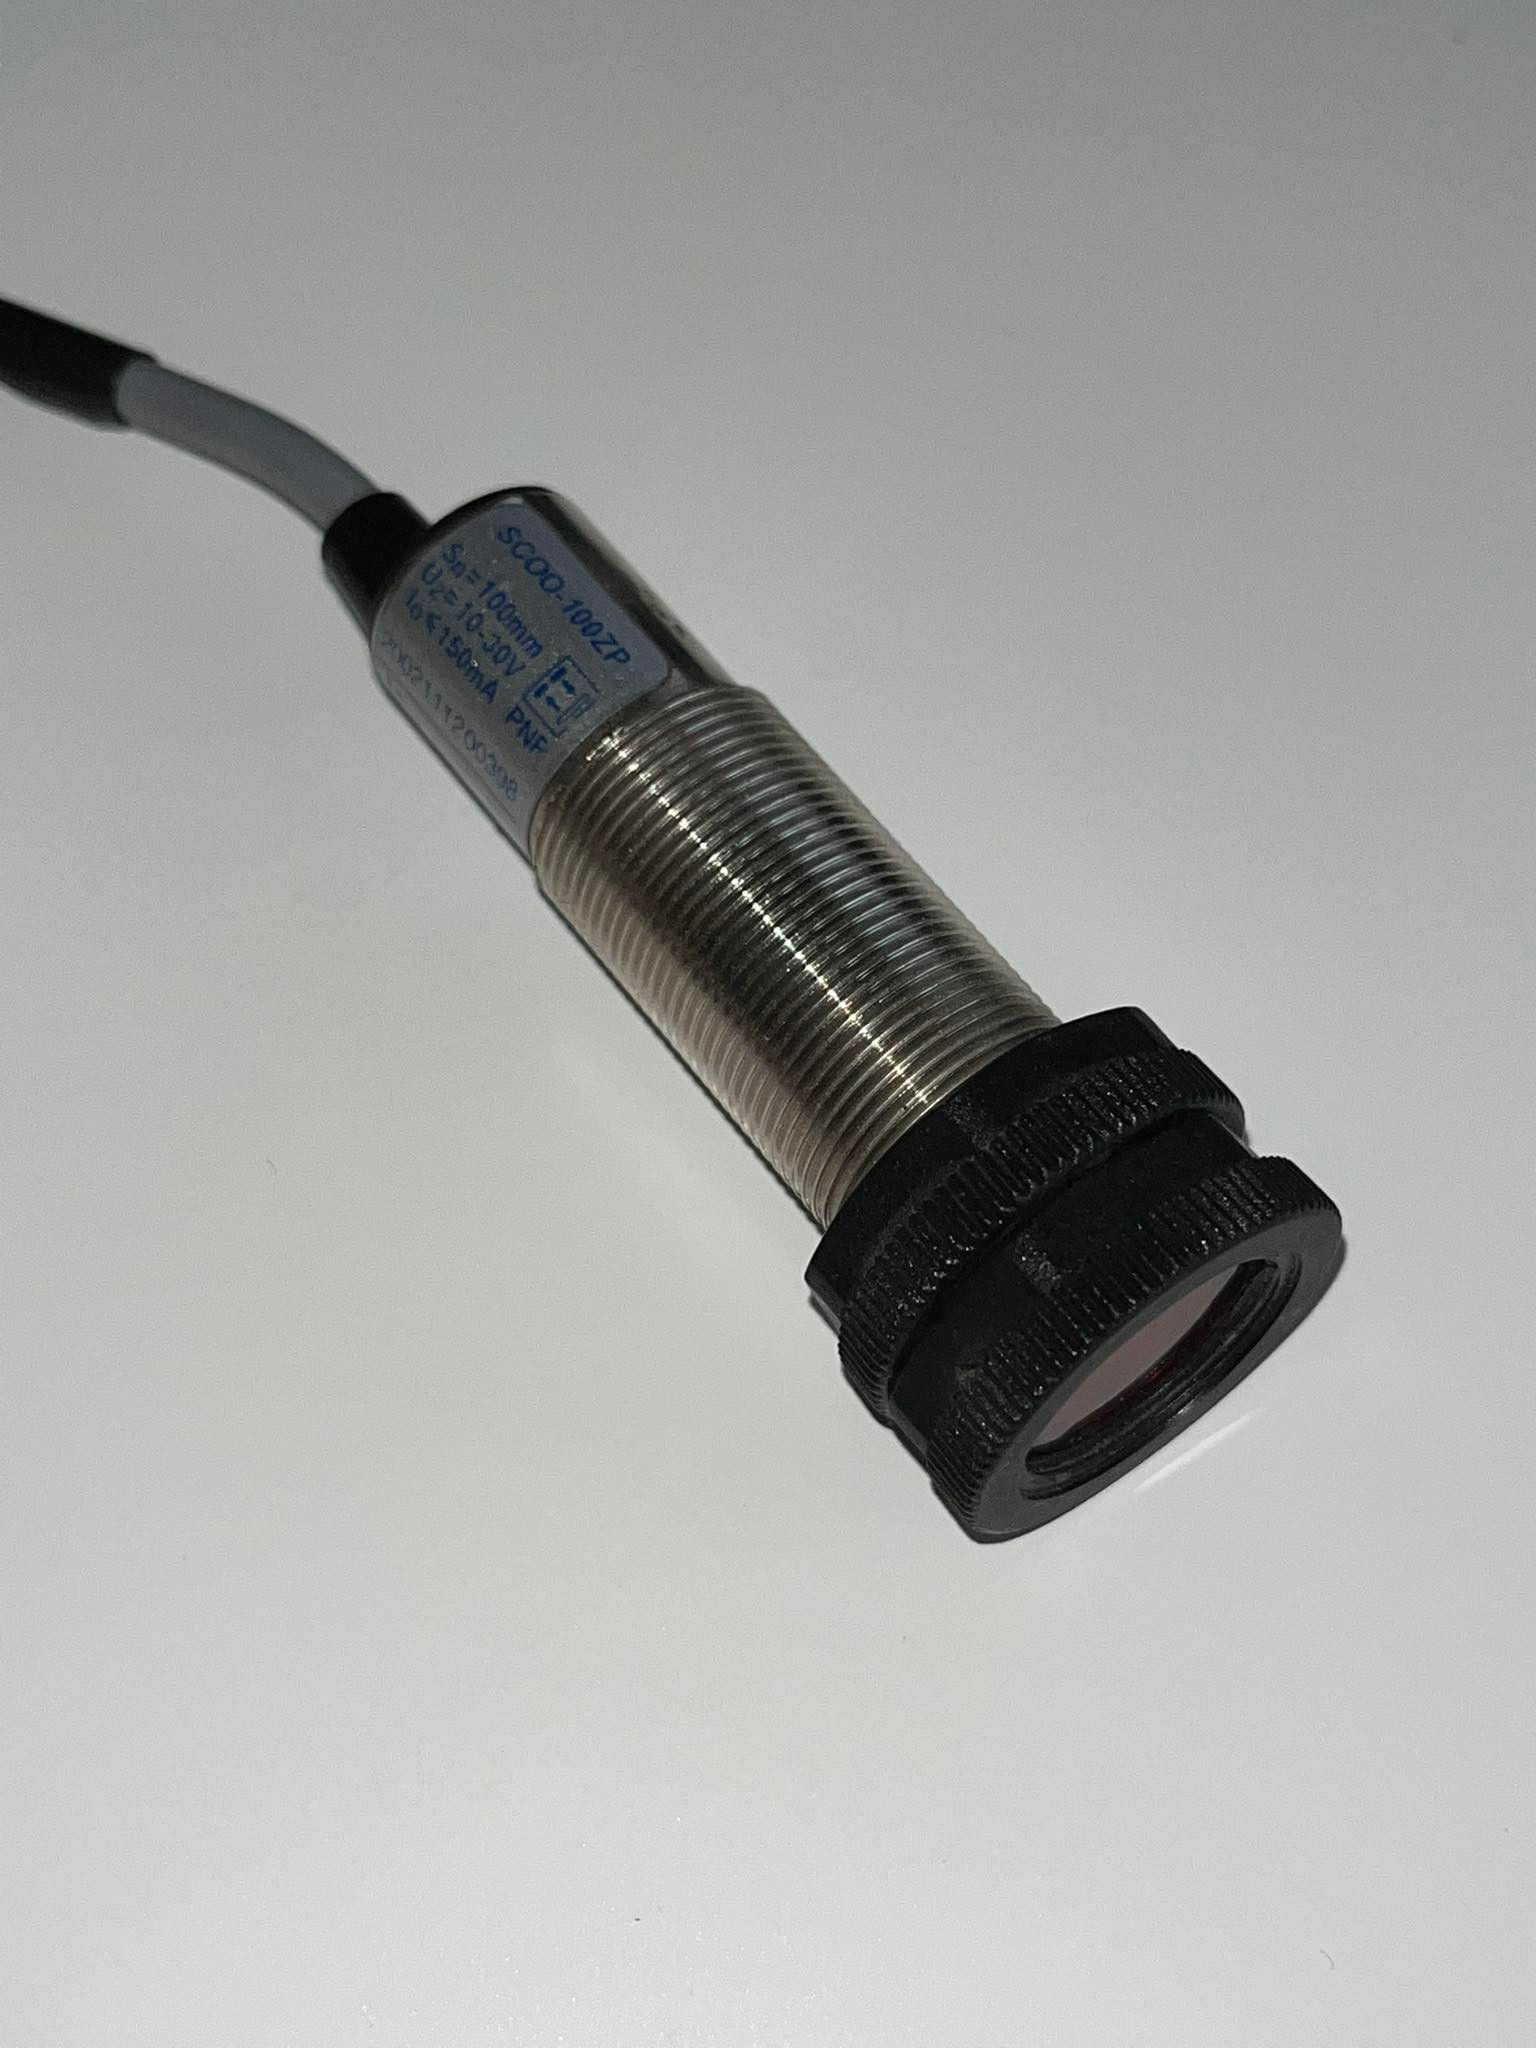
\includegraphics[width=.7\linewidth]{fig/SCOO/czujnik.jpg}
\caption{Zdjęcie modułu}
\label{fig:_zdjecie_modulu}
\end{subfigure}%
%%%%%%%%%%%%%%%%%%%%%%%%%%%%%%%%%%%%%%%%%%%%%%%%%%%%%%%%%%%%%%%%%%%%%%%%%%%%%%%%%
\begin{subfigure}{.5\textwidth}
\centering
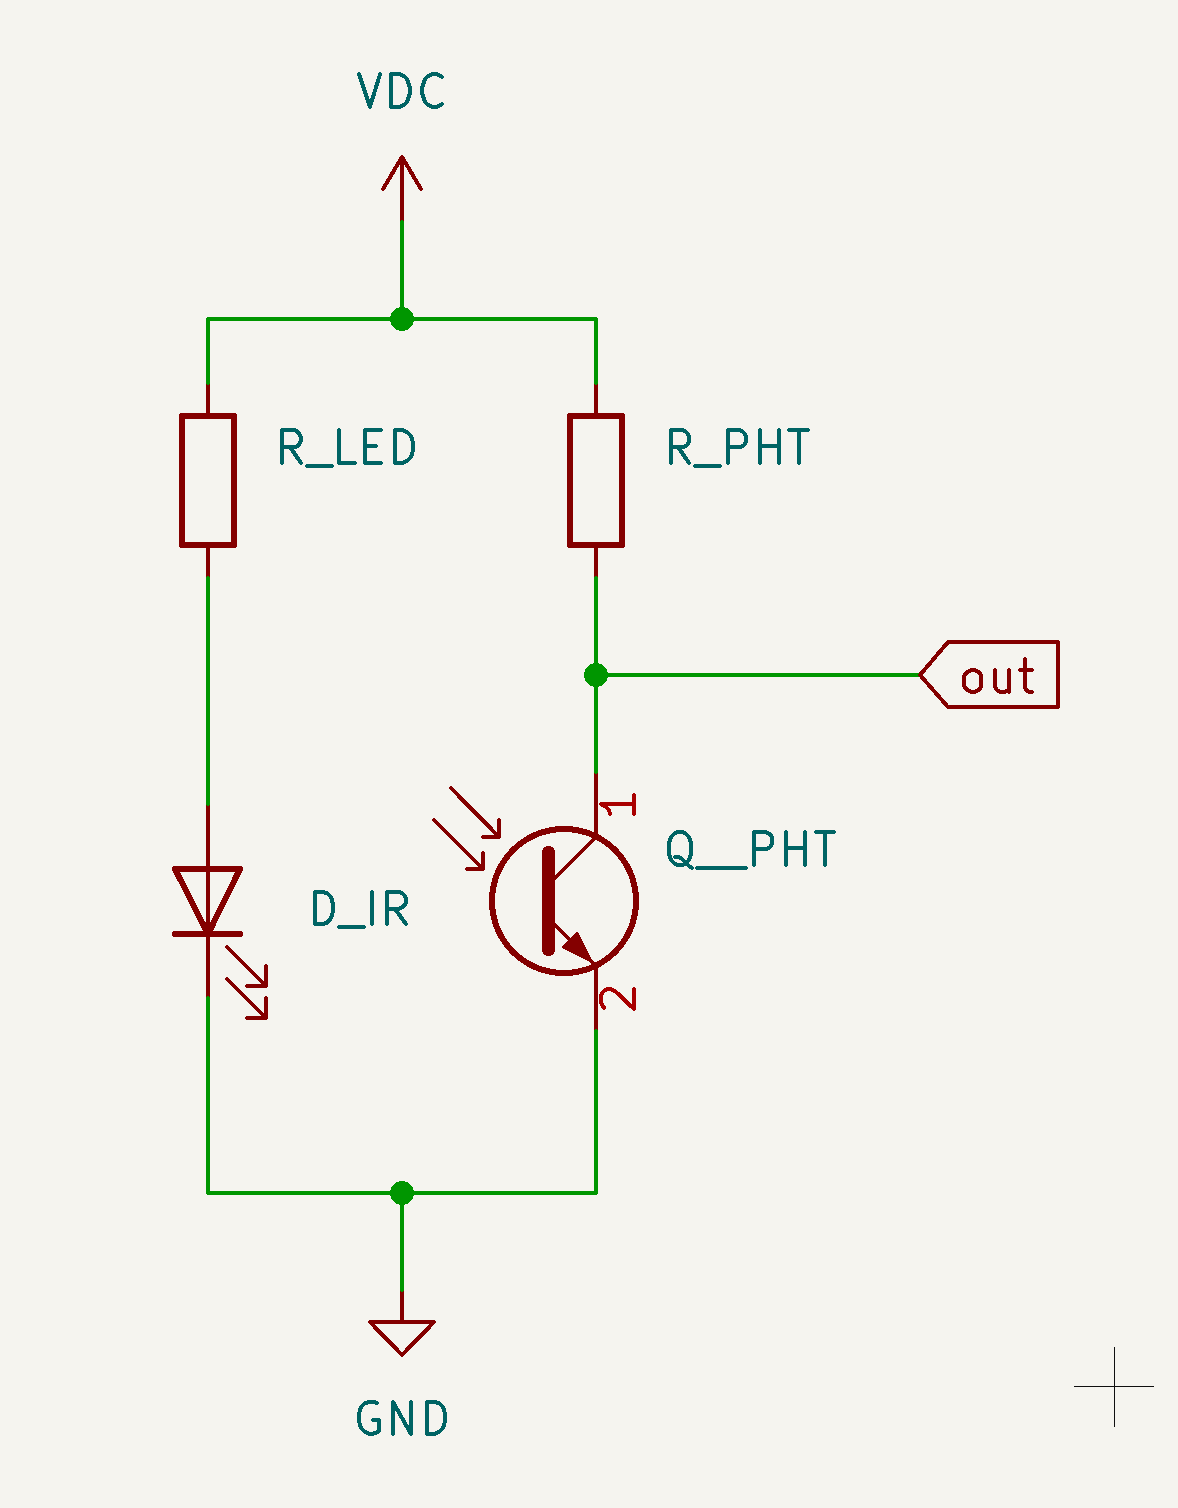
\includegraphics[width=.7\linewidth]{fig/SCOO/sche.png}
\caption{Schemat modułu}

\end{subfigure}
%%%%%%%%%%%%%%%%%%%%%%%%%%%%%%%%%%%%%%%%%%%%%%%%%%%%%%%%%%%%%%%%%%%%%%%%%%%%%%%%%
\label{fig:modul}
\end{figure}
\vspace{0.5cm}
%%%%%%%%%%%%%%%%%%%%%%%%%  TWO IMAGES SIDE BY SIDE  %%%%%%%%%%%%%%%%%%%%%%%%%%%%%

\newpage

\section{Użycie czujnika}
\subsection{Bez mikrokontrolera}

Działanie czujnika w trybie wyjścia progującego możemy zweryfikować, bez użycia mikrokontrolera, podłączając zasilanie w zakresie \texttt{10-30}V, oraz mierząc napięcie pomiędzy pinem \texttt{GND} oraz \texttt{OUT}.

\begin{figure}[h!]
    \centering
    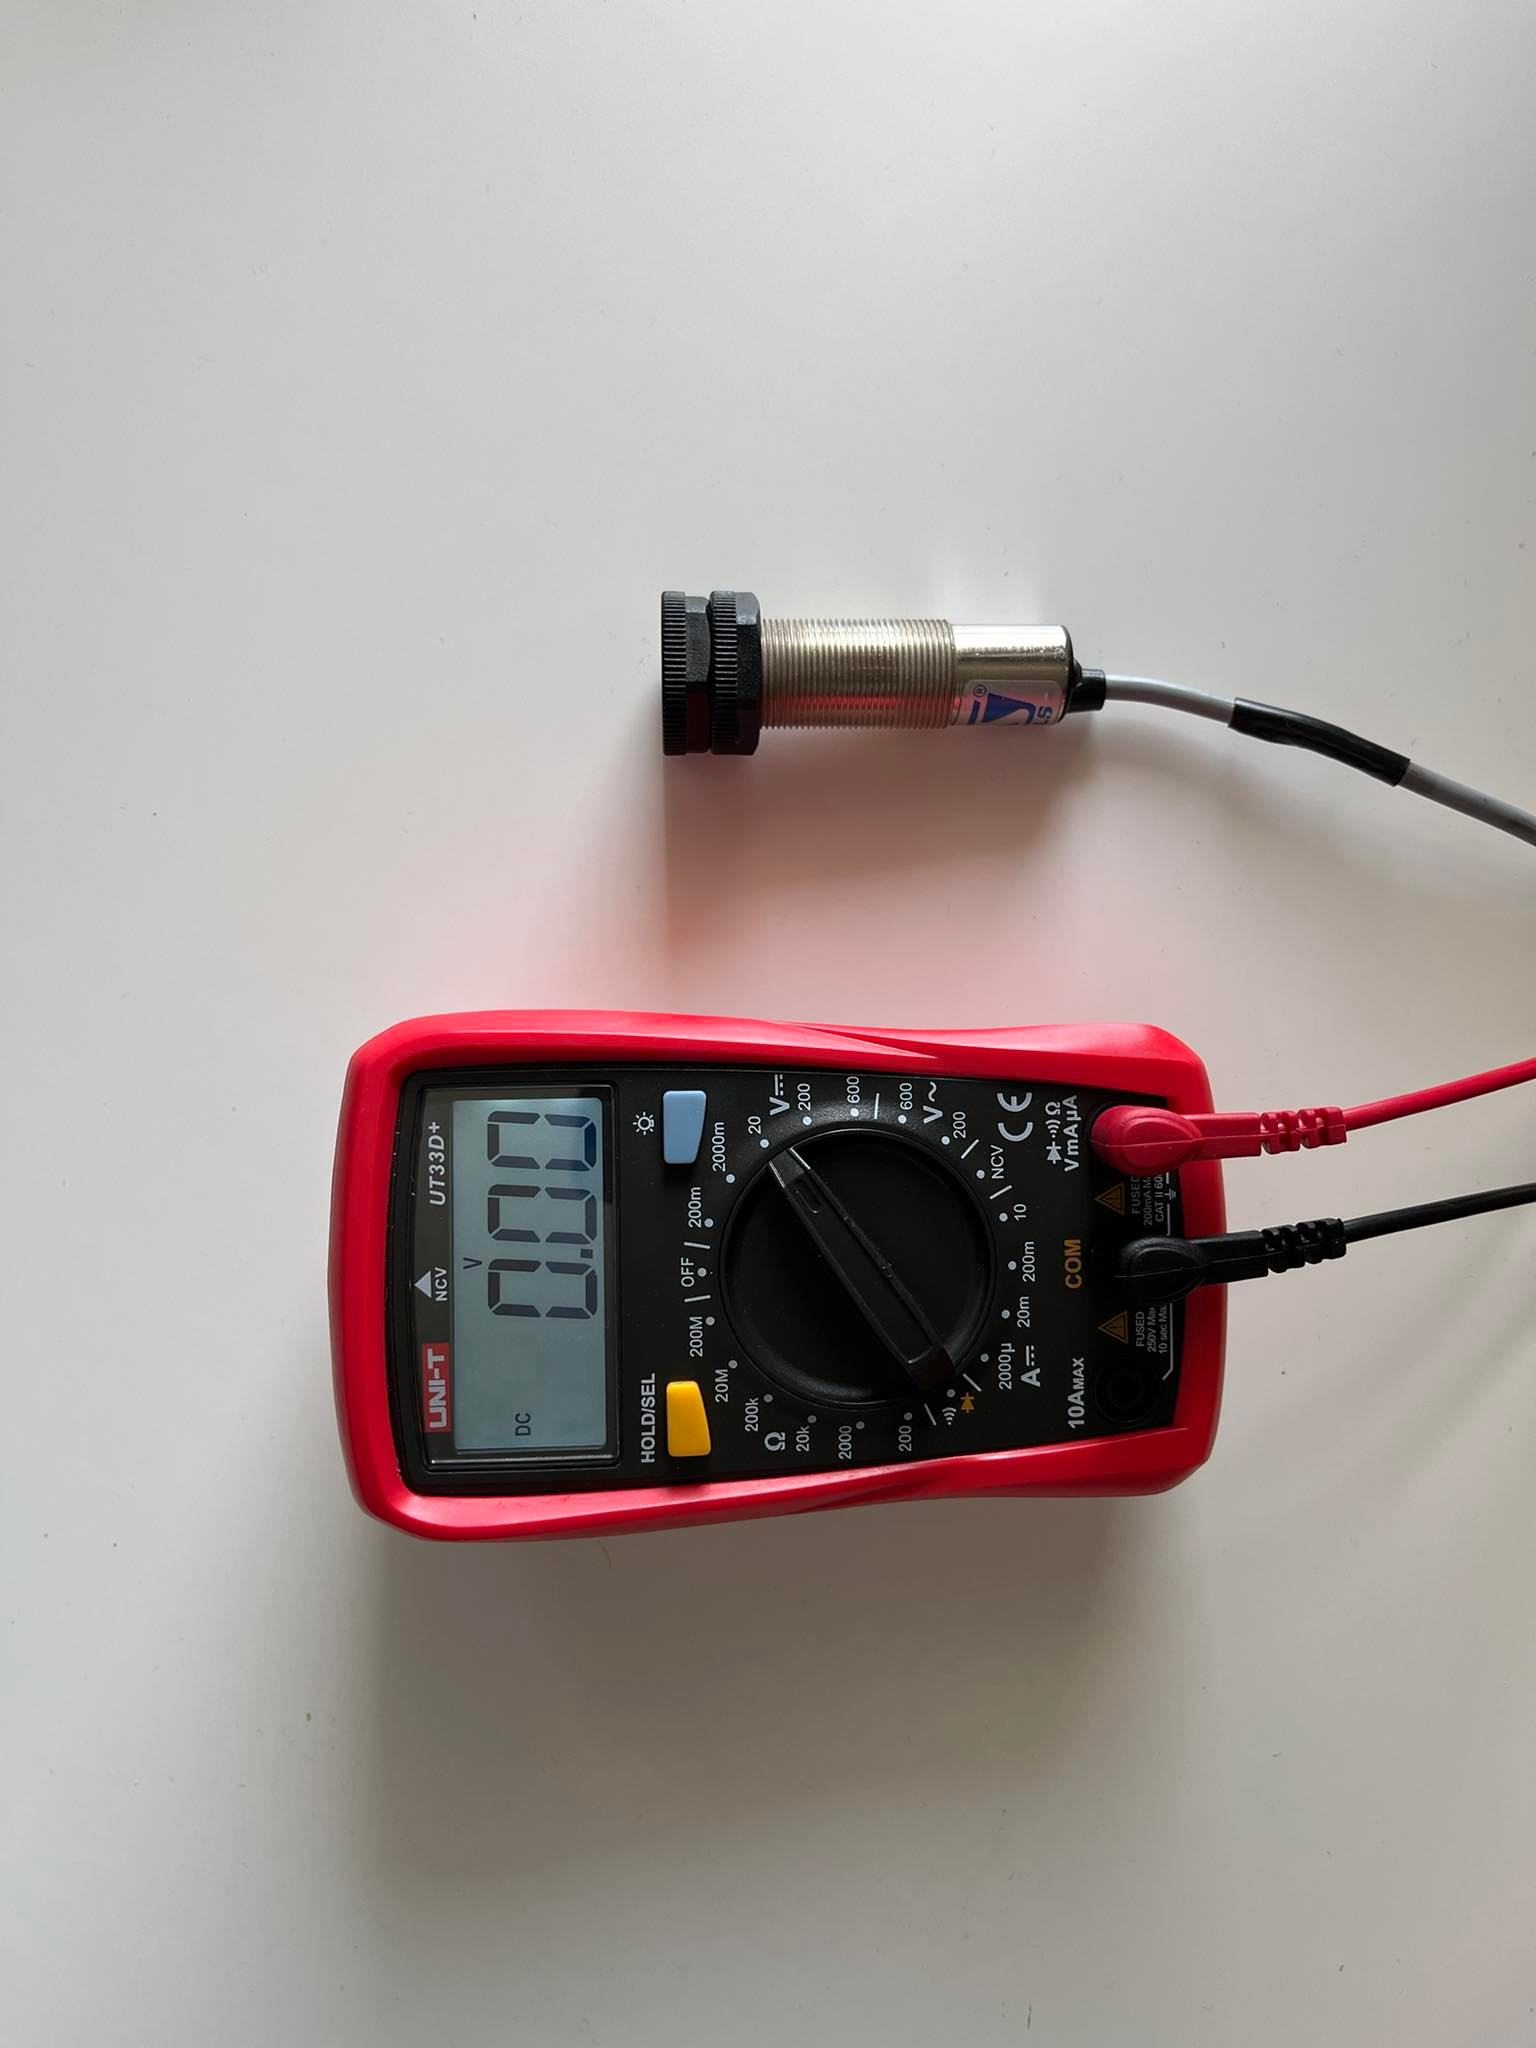
\includegraphics[angle=-90, width=0.7\textwidth]{fig/SCOO/stnd1-off.jpg}
    \caption{Brak wykrywanego elementu. $V_{out} = 0V$}
\end{figure}

\begin{figure}[h!]
    \centering
    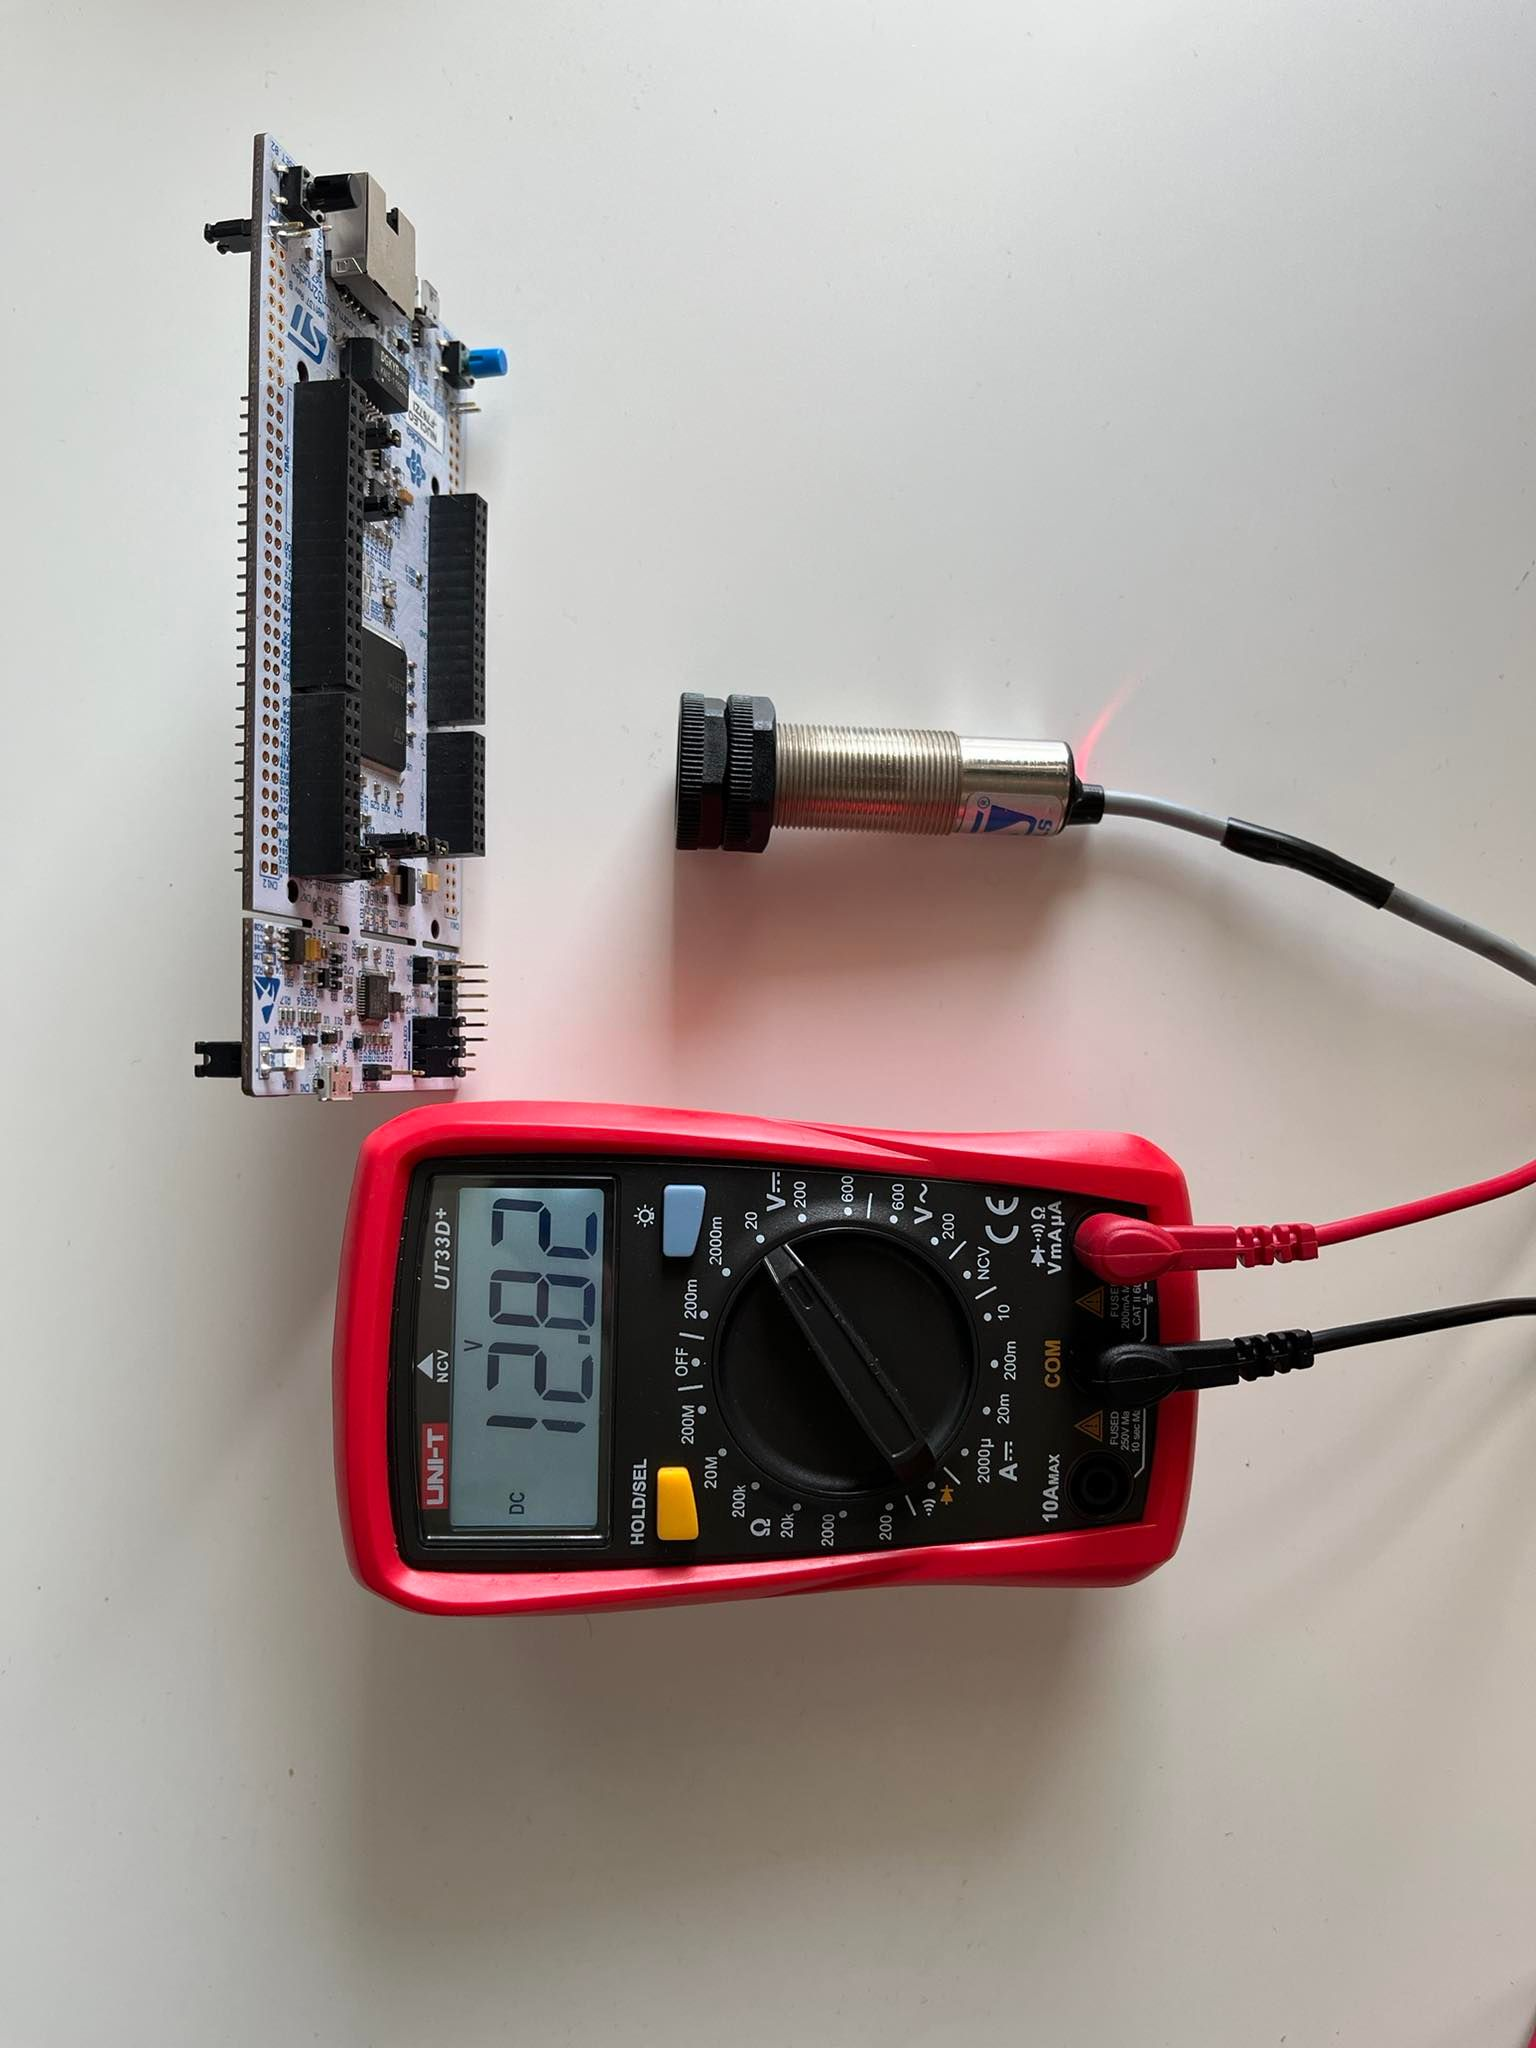
\includegraphics[angle=-90, width=0.7\textwidth]{fig/SCOO/stnd1-on.jpg}
        \caption{Wykrycie elementu. $V_{out} = V_{dc}$}
\end{figure}

\newpage

\begin{figure}[h!]
    \centering
    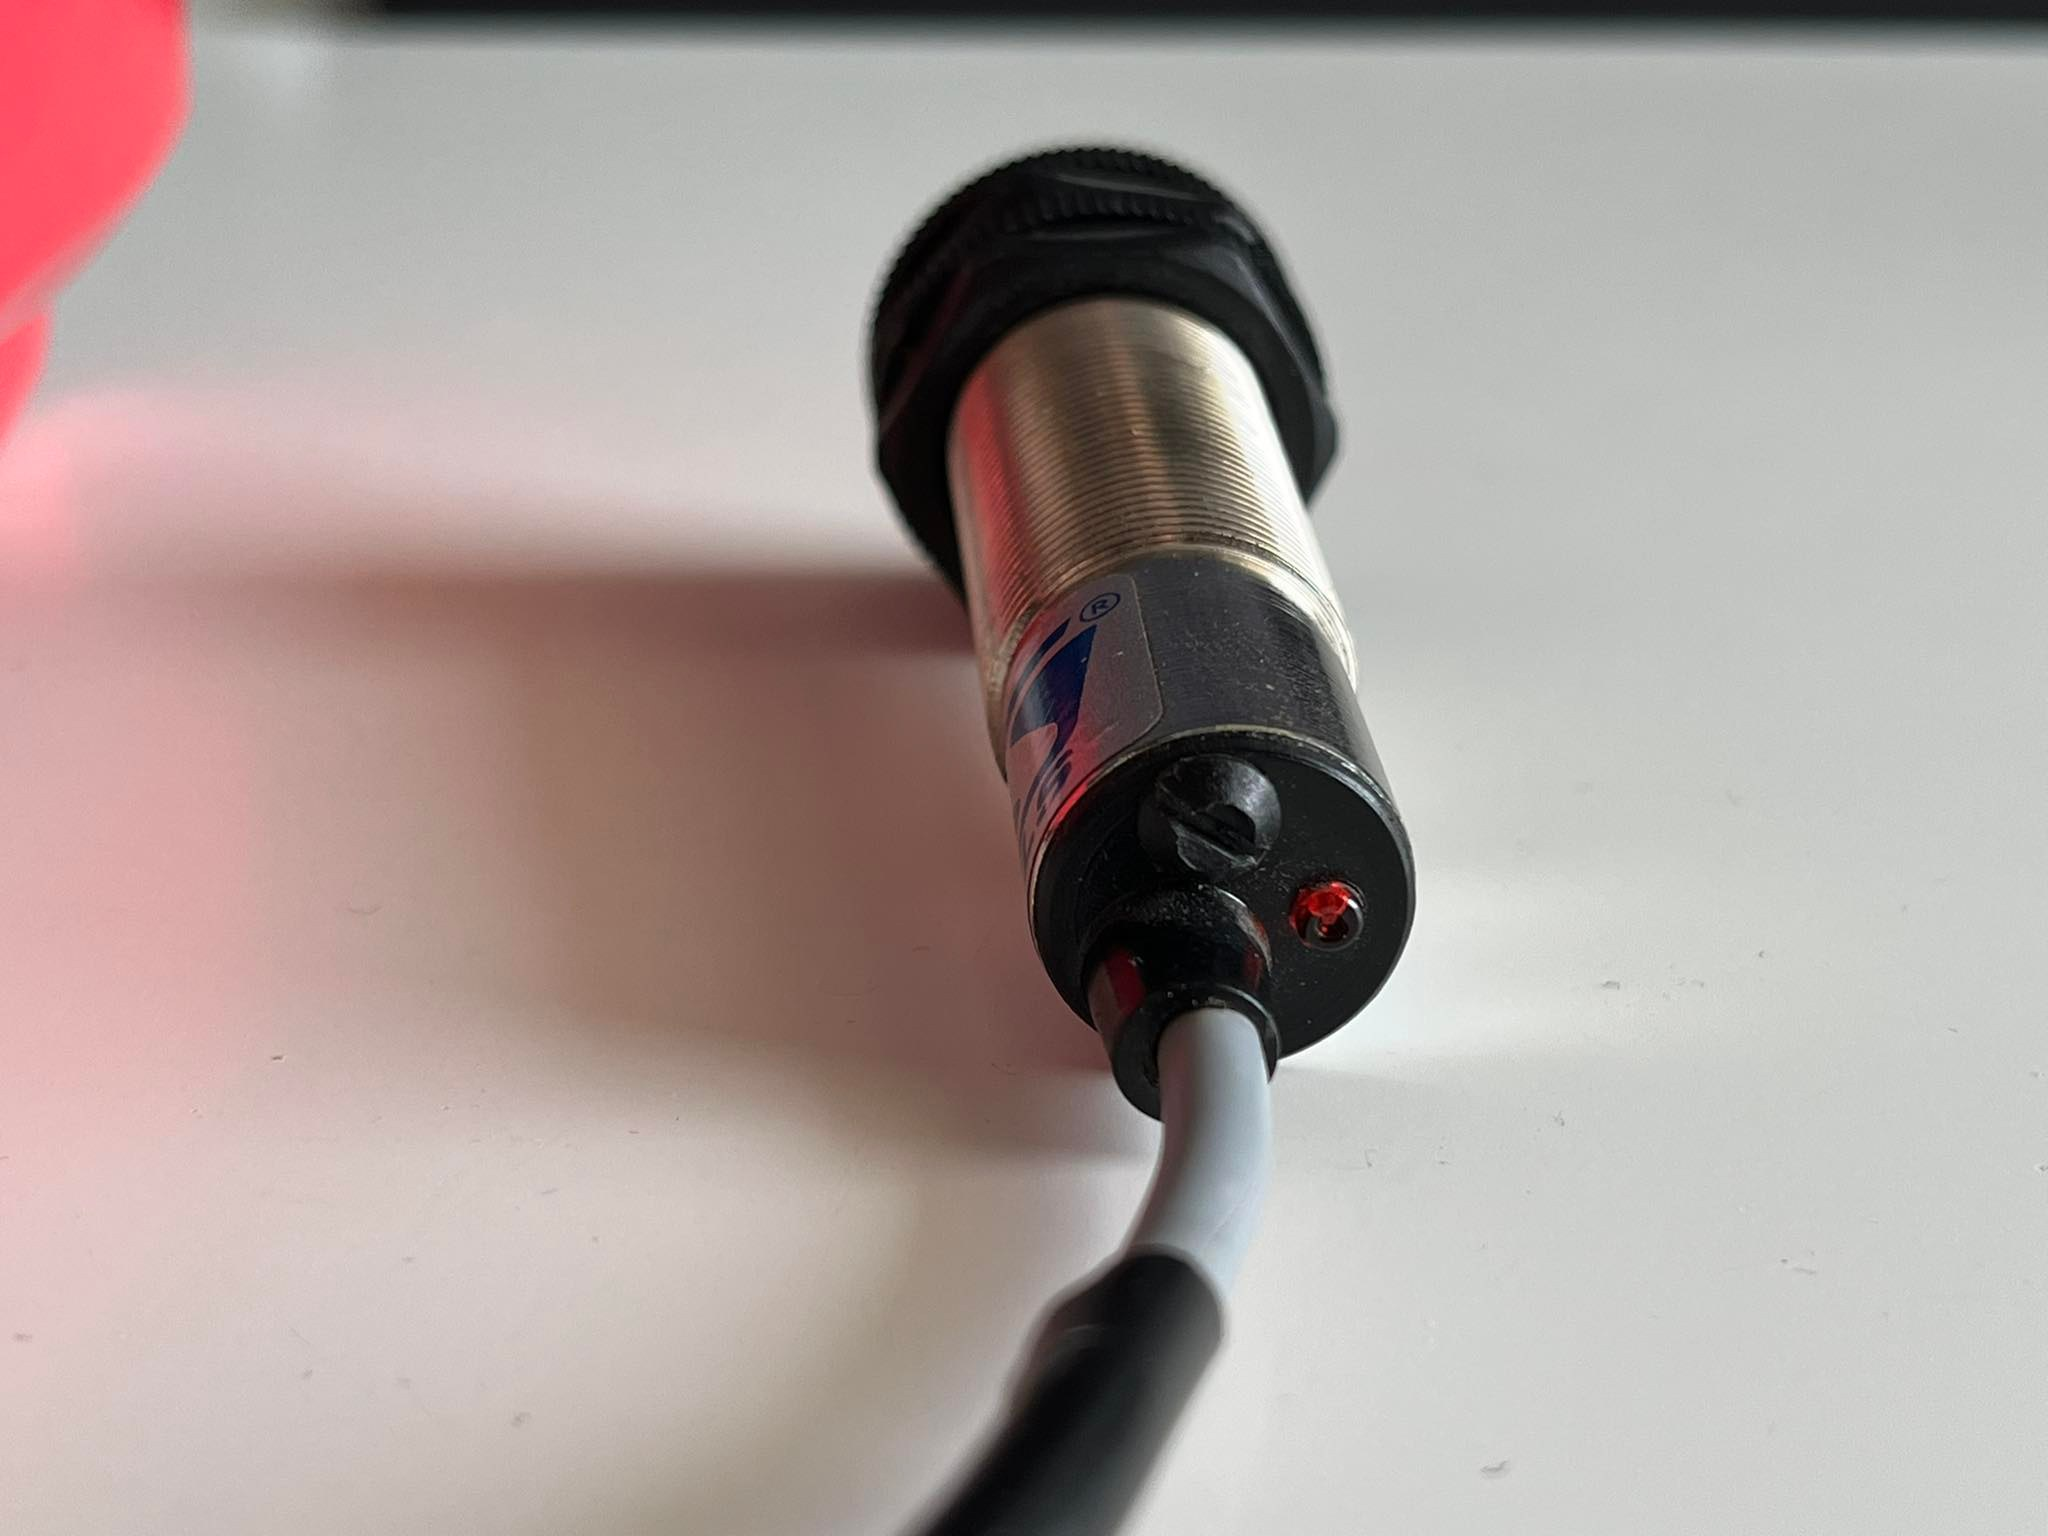
\includegraphics[angle=0, width=0.7\textwidth]{fig/SCOO/stnd2-off.jpg}
    \caption{Brak wykrywanego elementu. Dioda statusu wyłączona}
\end{figure}

\begin{figure}[h!]
    \centering
    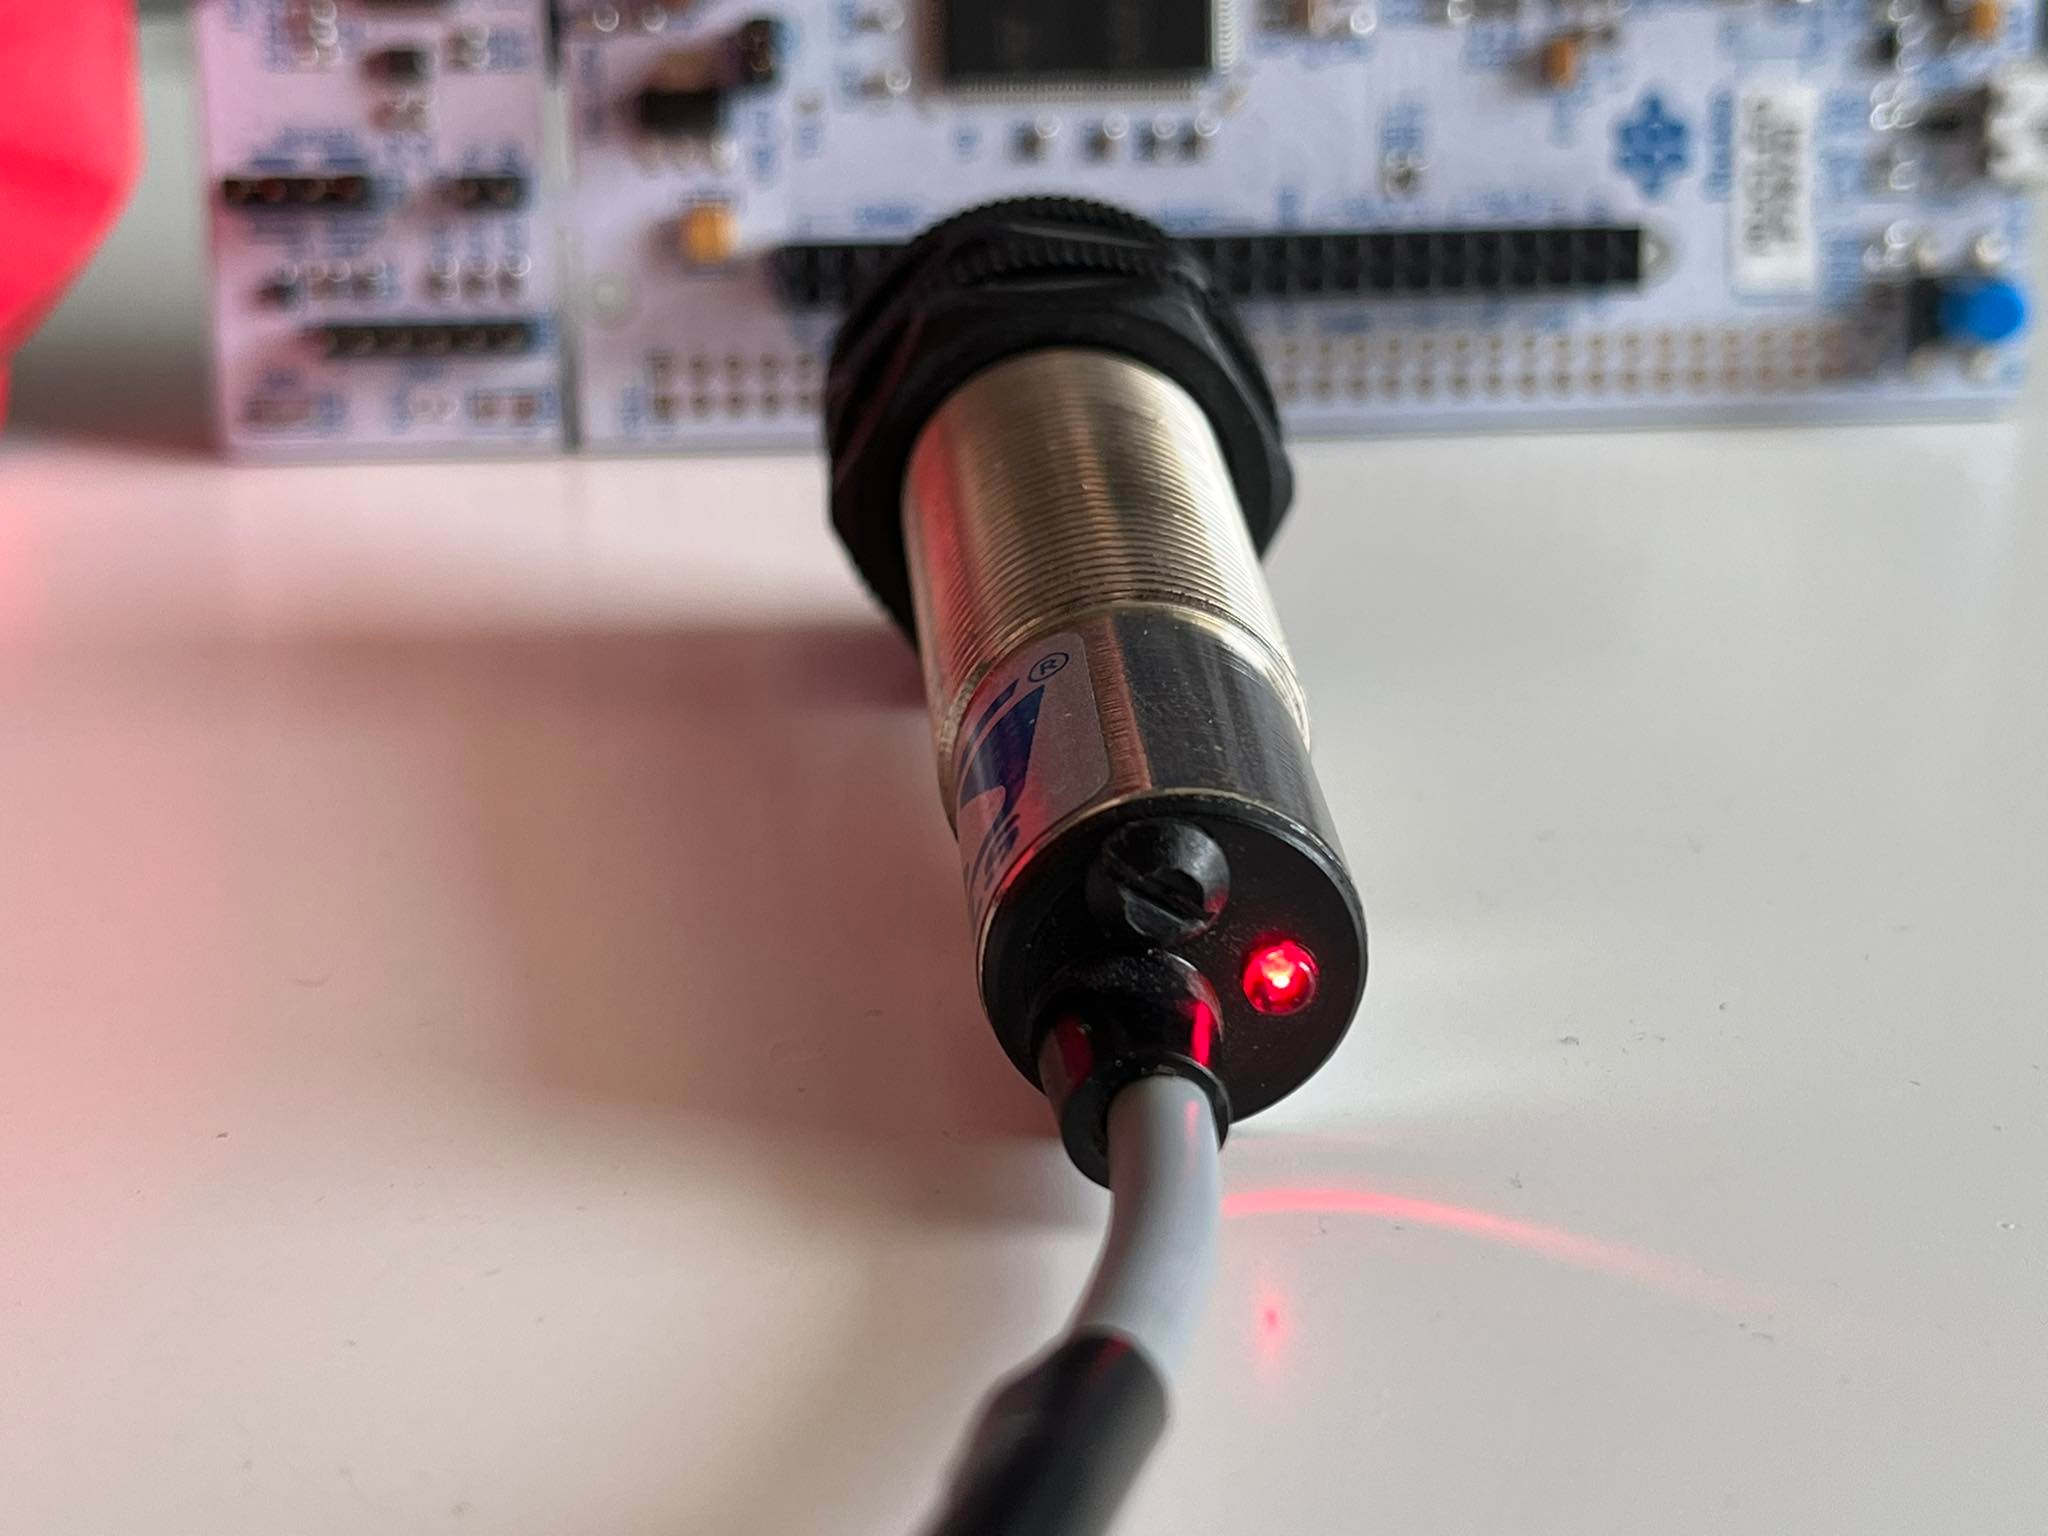
\includegraphics[angle=0, width=0.7\textwidth]{fig/SCOO/stnd2-on.jpg}
    \caption{Wykrycie elementu. Dioda statusu włączona}
\end{figure}

\newpage
\subsection{Mikrokontroler}
Oczywiście czujnik możemy używac w połączeniu z mikrokontrolerem. Schemat połączeń i konfiguracja
mikrokontrolera została opisana w sekcji \texttt{Suplement \#1}.Zawiera tam się również kod języka
C + HAL, pozwalający odczytać wartości z czujnika.

Należy zwrócić jednak uwagę na występowanie dodatkowego dzielnika napięć. Jest to wymagane aby obniżyć poziom logiczny wyjścia
czujnika z $V_{dc}$, do poziomu akceptowalnego przez mikro-kontroler $V_{out} \le 3.3V$.

\begin{figure}[h!]
    \centering
    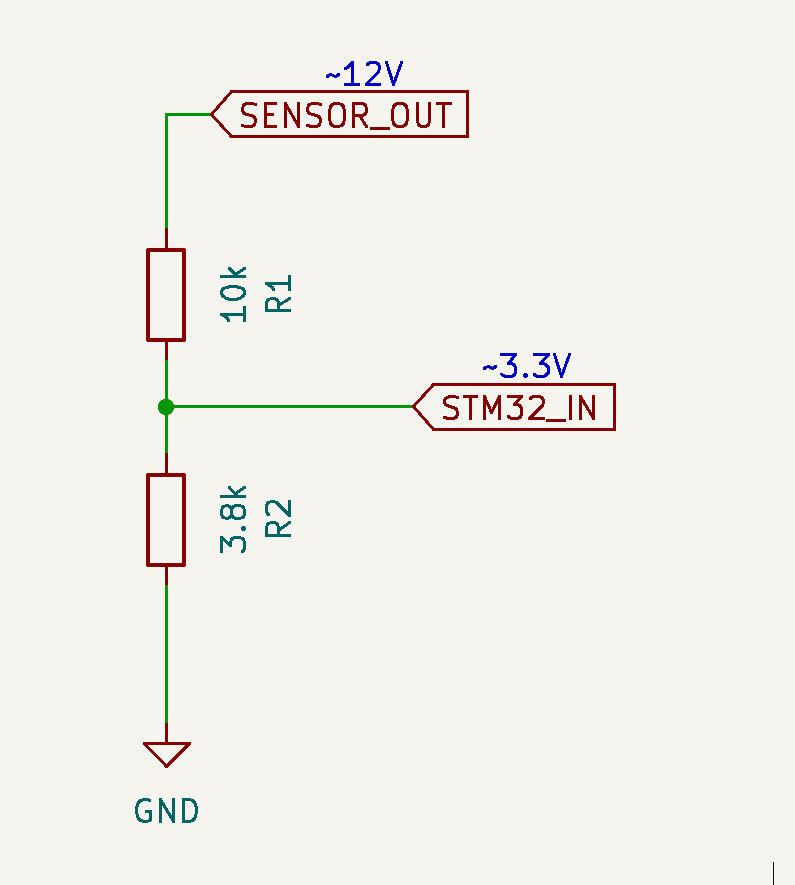
\includegraphics[width=0.4\textwidth]{fig/SCOO/res.png}
    \caption{Schemat dzielnika napięć}
\end{figure}


\begin{figure}[h!]
    \centering
    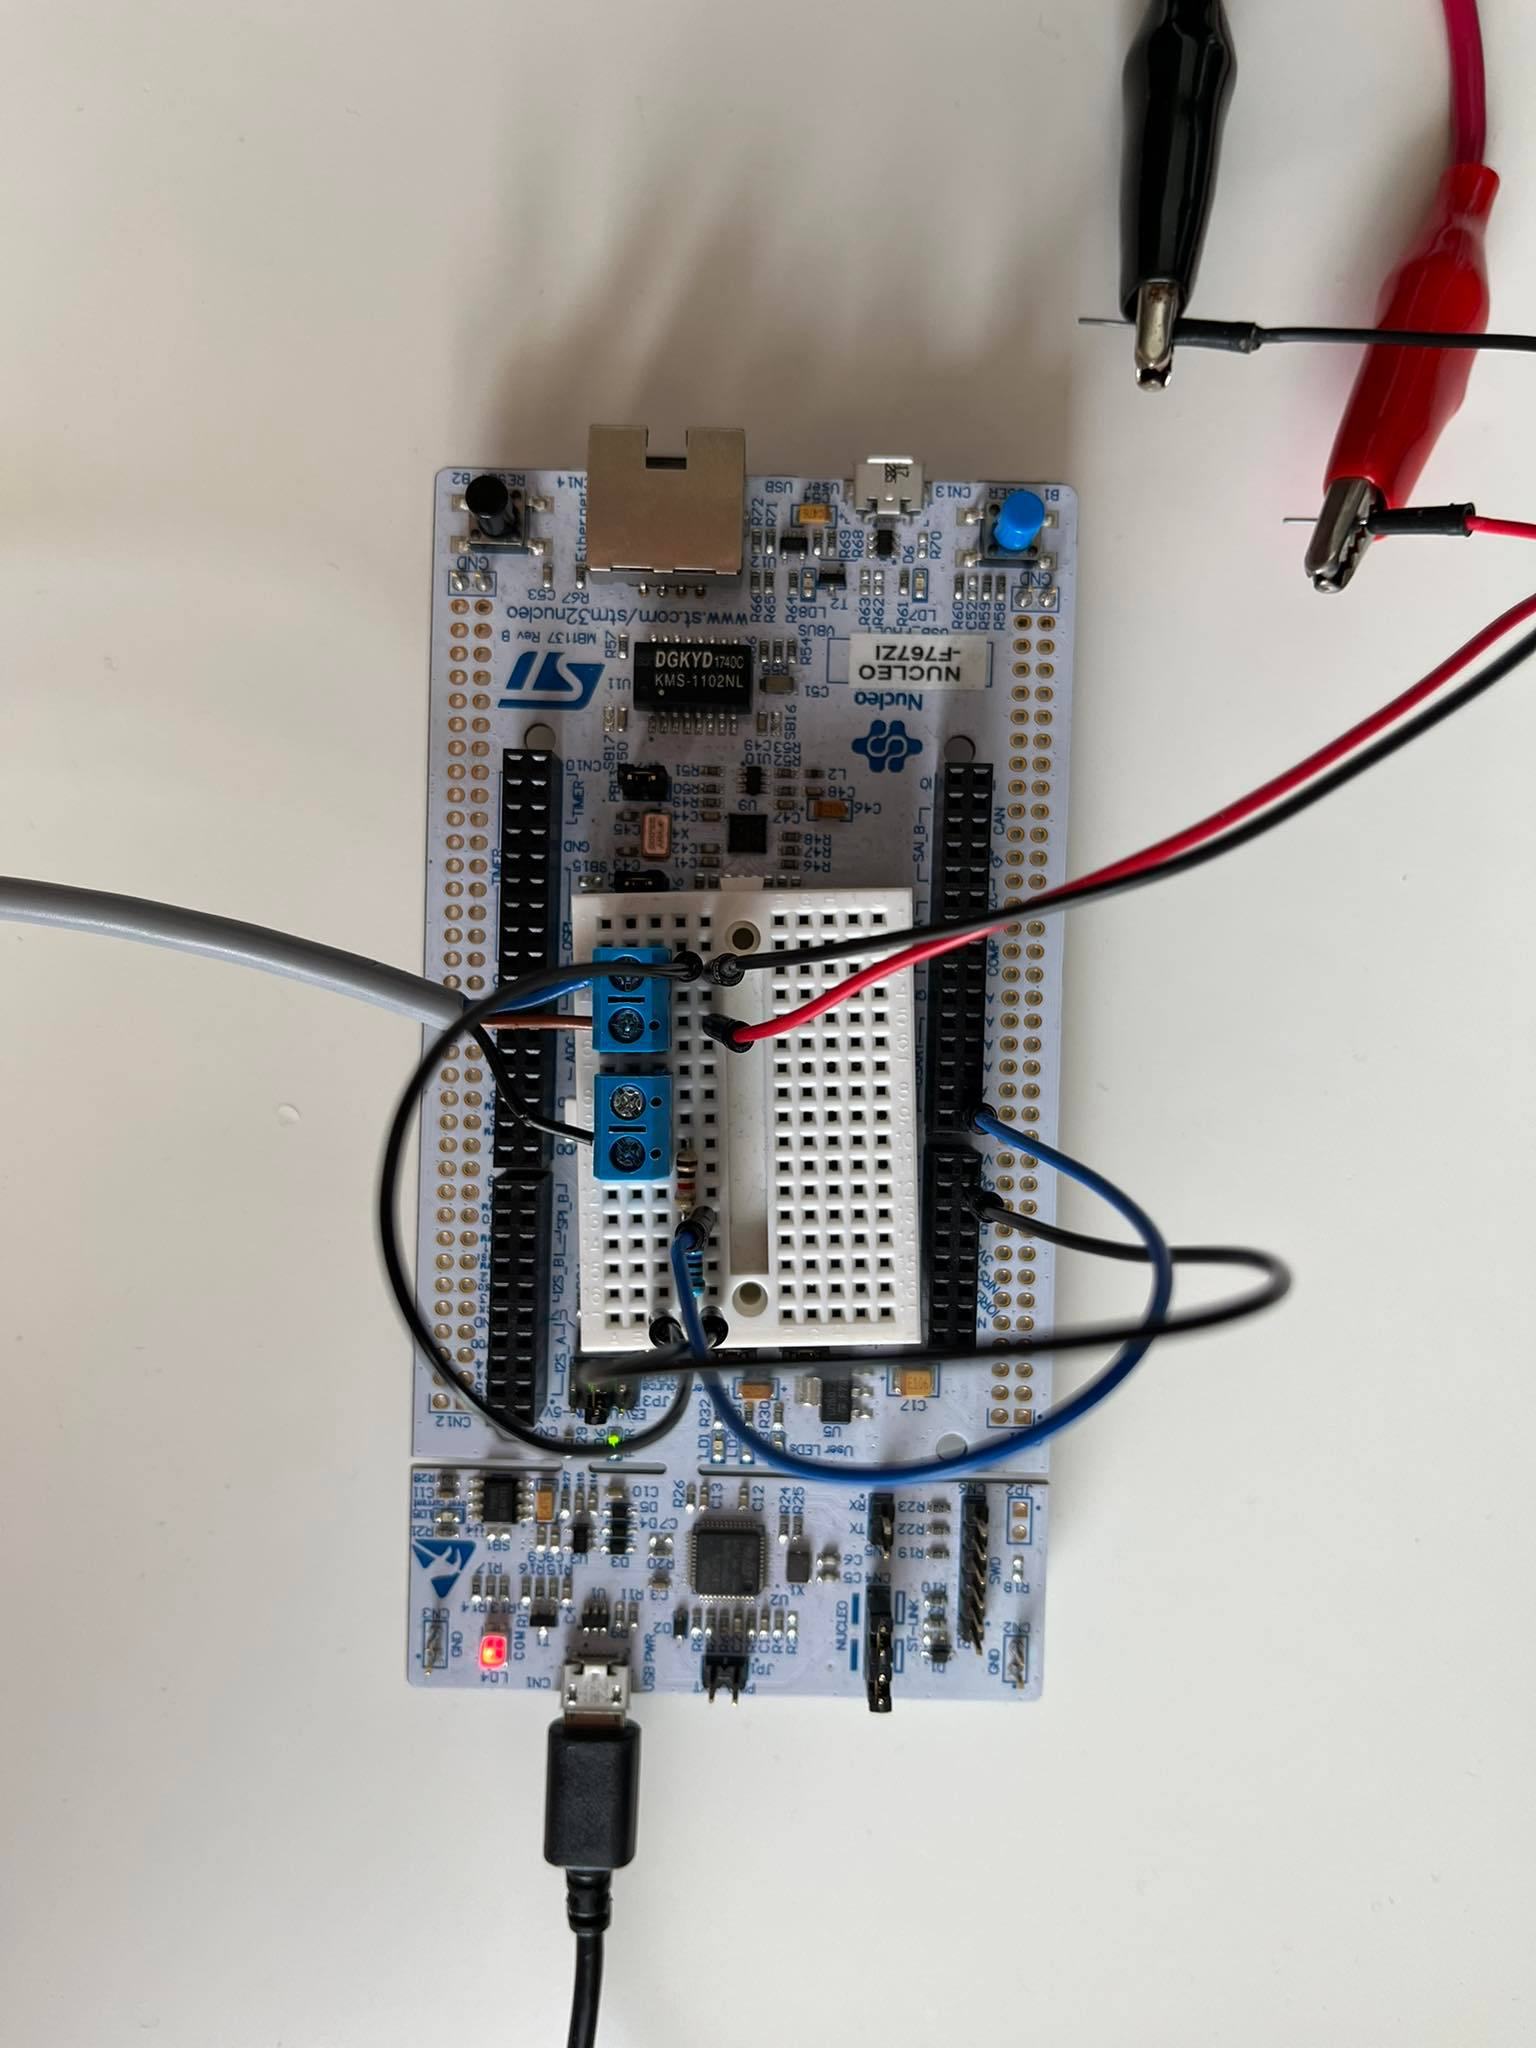
\includegraphics[angle=90, width=0.7\textwidth]{fig/SCOO/pol1.jpg}
    \caption{Połączenie z mikokontrolerem. Należy zwrócić uwagę na zwarcie mas czujnika i mikrokontrolera}
\end{figure}

\newpage

Kod jest skonfigurowany tak, aby uruchamiał wbudowany w płytkę mikrokontrolera element LED. Na 
zdjęciach dodatkowo widać działanie wbudowanej w moduł diody LED. 

\begin{figure}[h!]
    \centering
    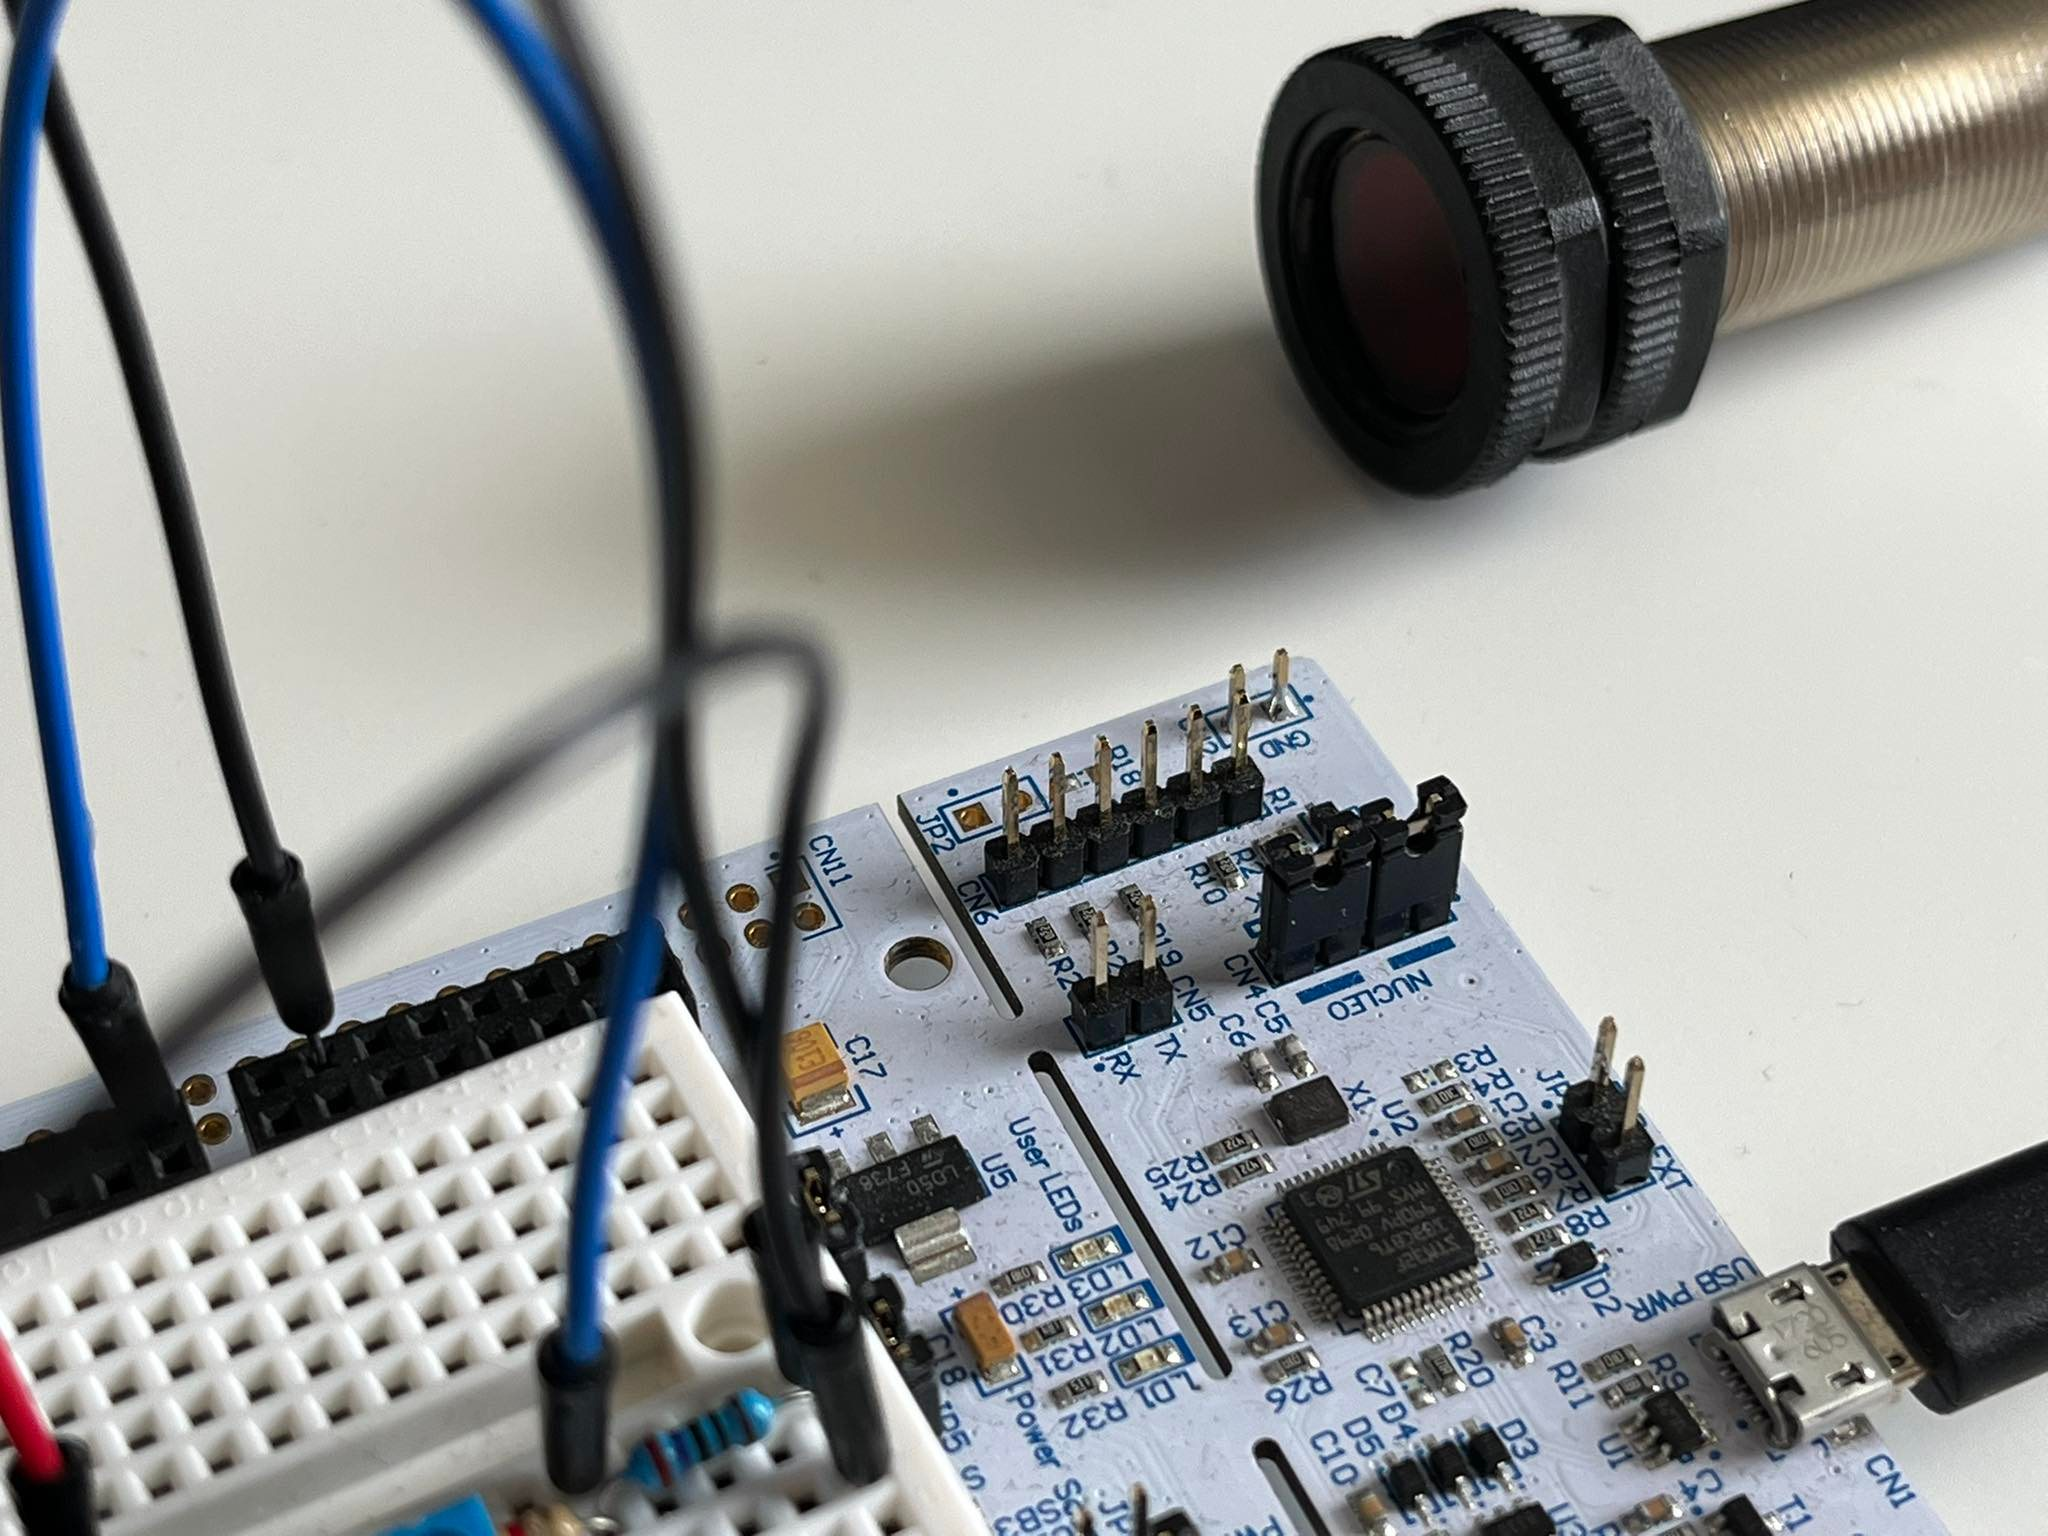
\includegraphics[angle=0, width=0.7\textwidth]{fig/SCOO/mikro-off.jpg}
    \caption{Brak wykrywanego elementu. \texttt{LD1} wyłączone}
\end{figure}

\begin{figure}[h!]
    \centering
    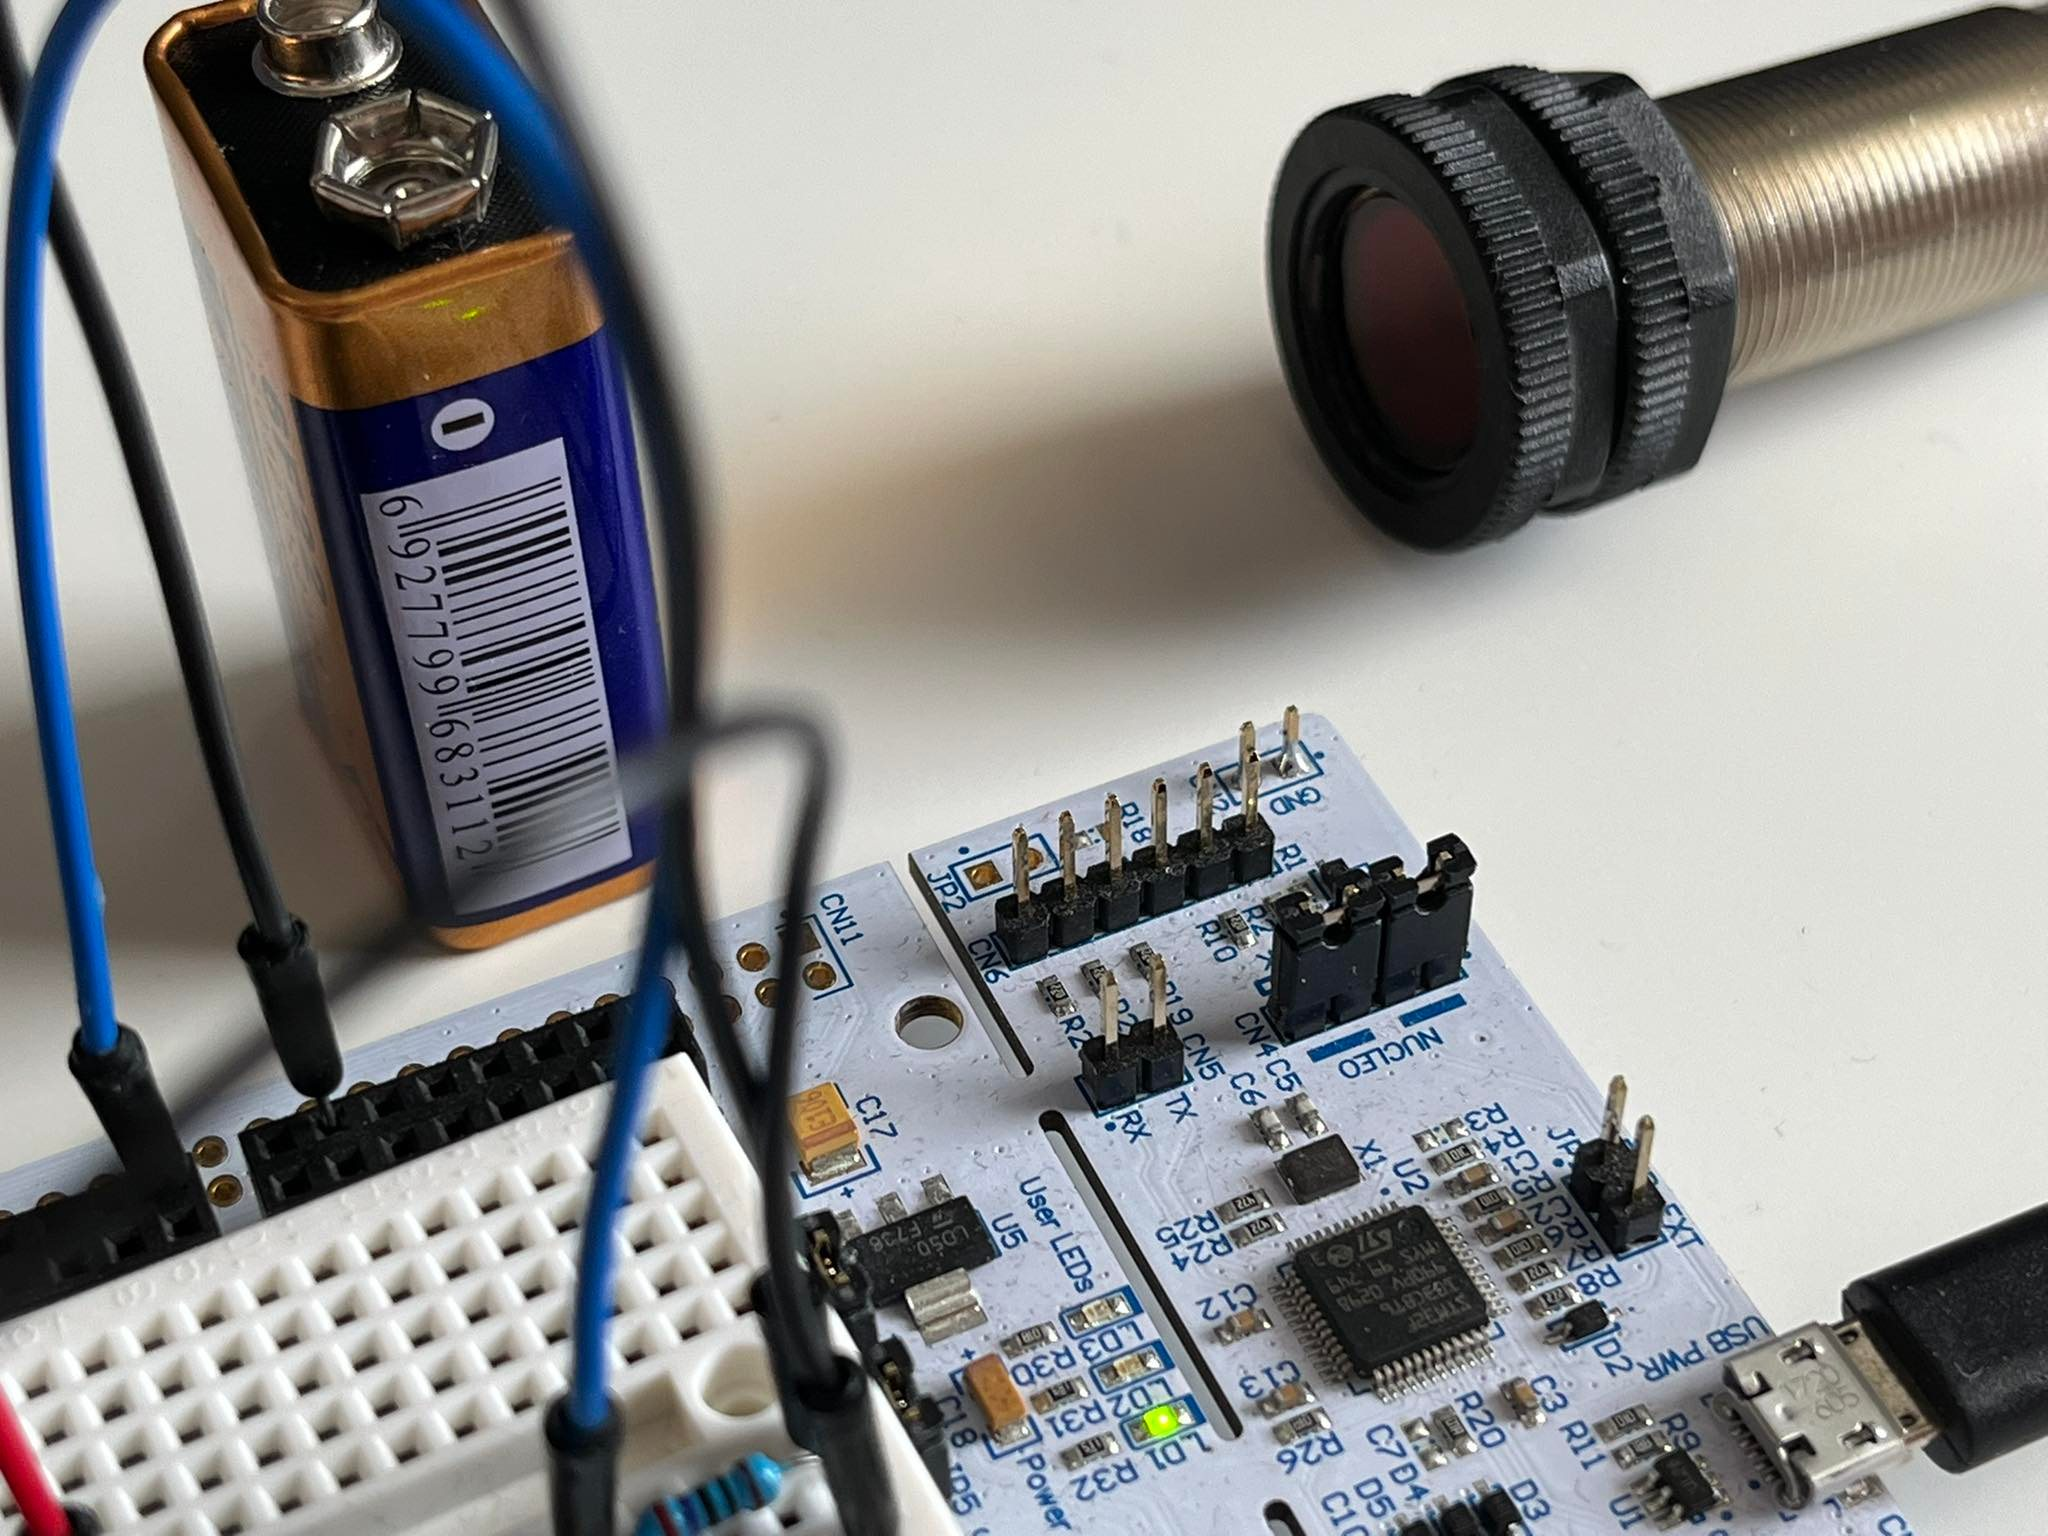
\includegraphics[angle=0, width=0.7\textwidth]{fig/SCOO/mikro-on.jpg}
        \caption{Wykrycie elementu. \texttt{LD1} włączone}
\end{figure}


\newpage
\printbibliography[heading=bibintoc]

\end{document}